\chapter{Architecture}
This chapter highlights the architecture of the Substitution Stepper as well as the reasoning for some big decisions.

\section{Overview}
The Substitution Stepper consists of multiple logically grouped folders that each have a specific responsibility.
The most important folders/modules are shown in Figure \ref*{fig:architecture},
though not all of them are shown in full detail as that would clutter up the diagram too much and would not provide a lot of value.

\begin{figure}[ht!]
    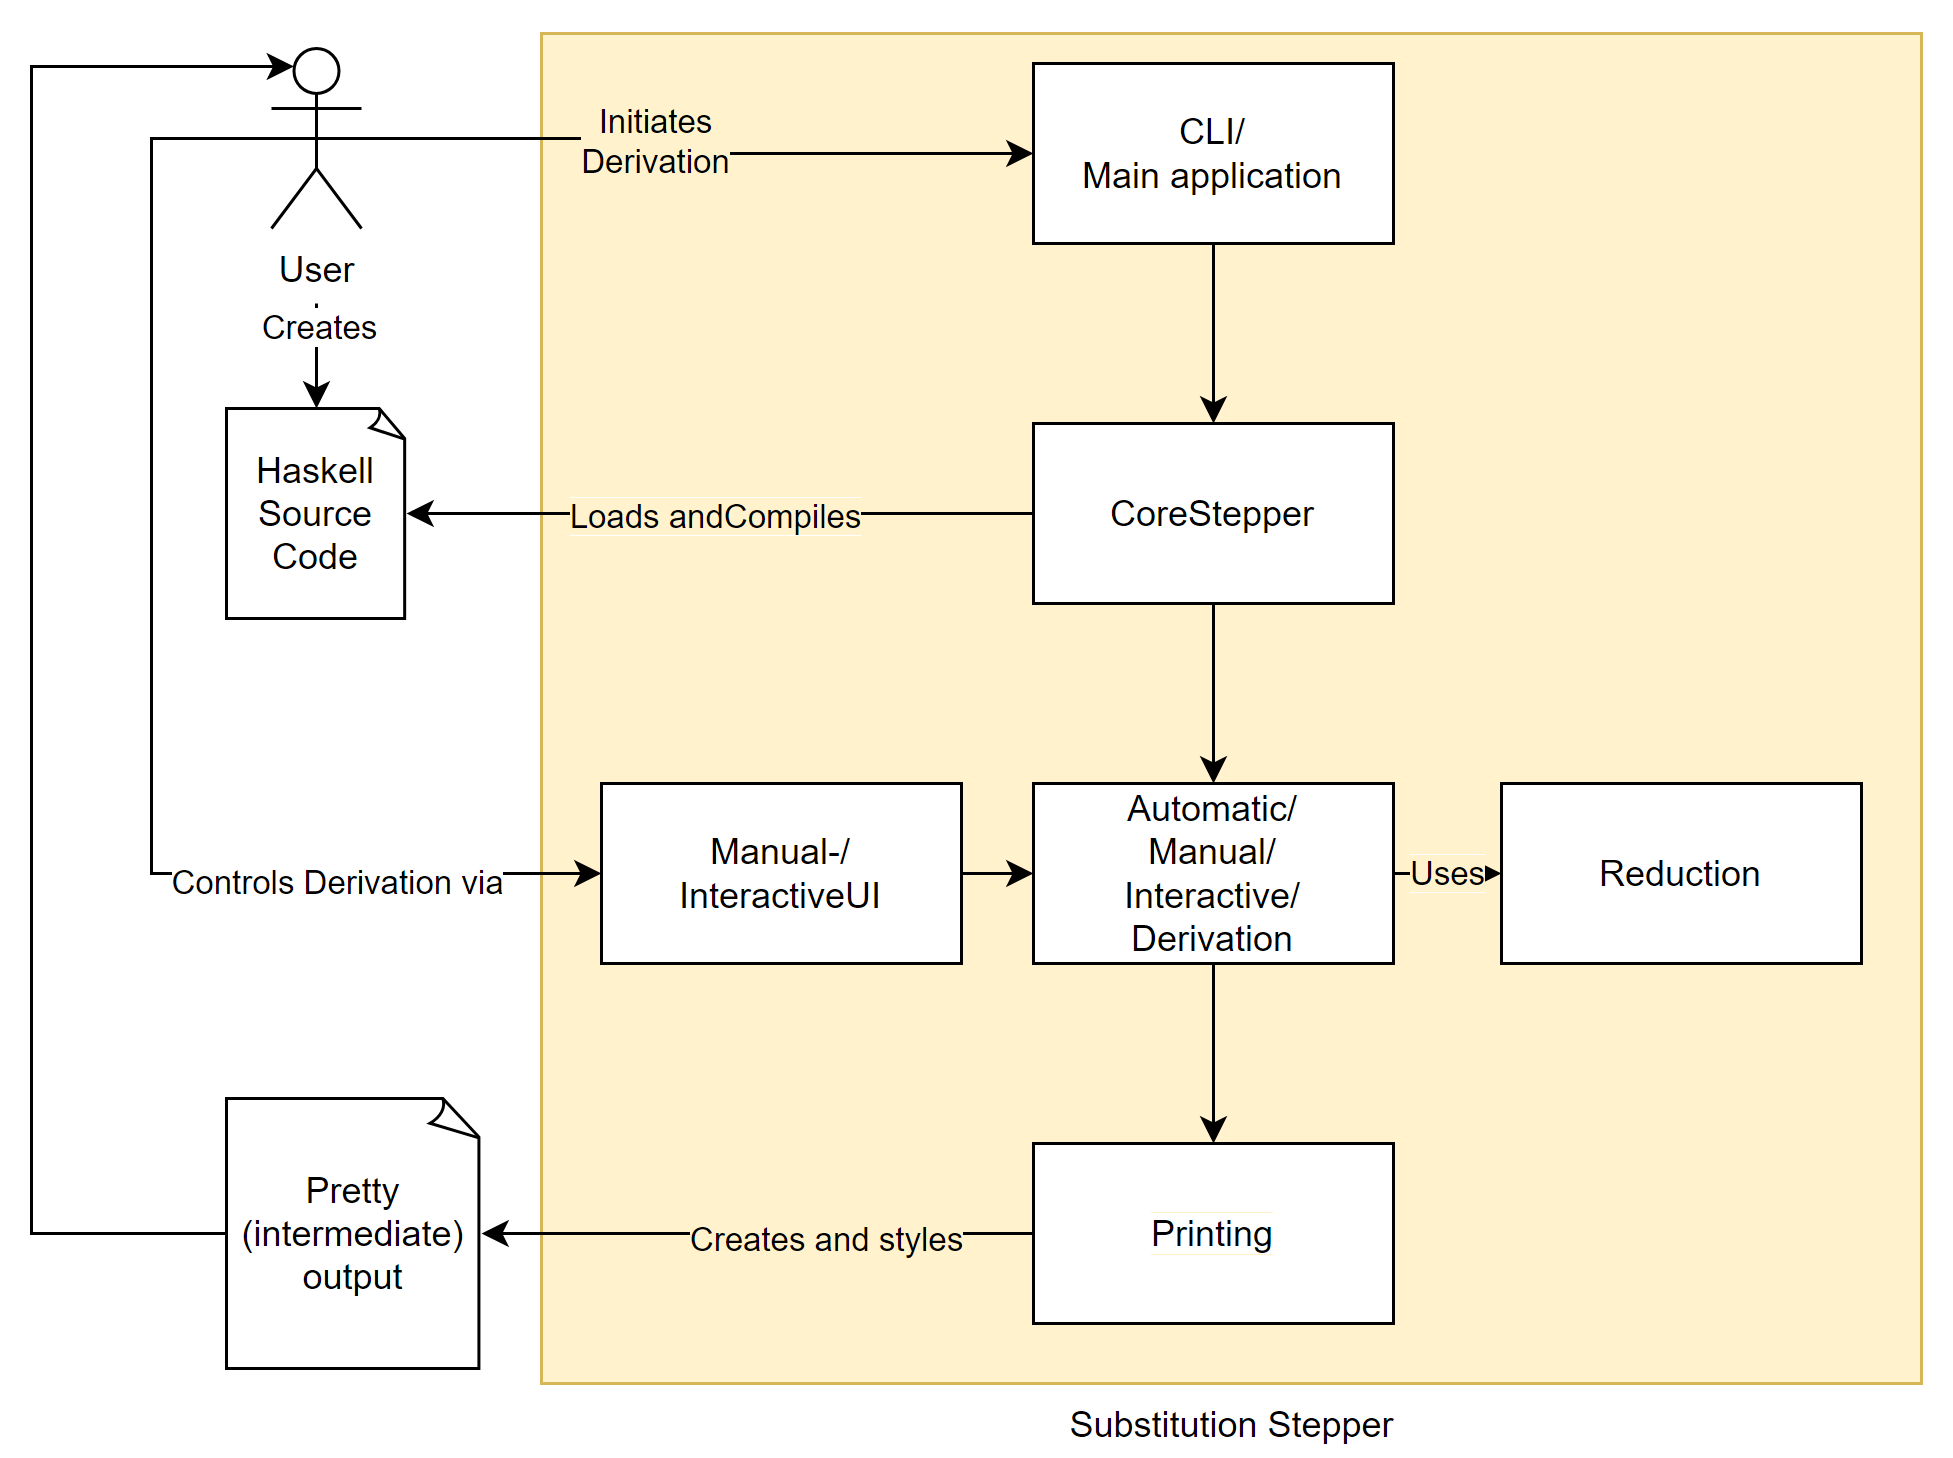
\includegraphics[width=1\textwidth]{resources/Architecture.PNG}
    \caption{Architecture of the Substitution Stepper}
    \label{fig:architecture}
\end{figure}

\subsection{Main application}
The main application is responsible for initiating the derivation.
The module AppConfig is used by the main application to extract the relevant arguments from the command line,
based on which the derivation is initiated.
The AppConfig module is also responsible for adding default values for arguments that were not passed to the application.

\subsection{CoreStepper}
The CoreStepper module, which was developed outside of the scope of this thesis,
takes Haskell source code and compiles it to GHC Core code.
All bindings from the stepped module are collected and returned.
The binding for the stepped function is fetched as well and passed to the Derivation module via the main application.

\subsection{Derivation}
The module \texttt{Derivation.DerivationUtils} is used by the main application to prepare the GHC Core code for stepping.
The function \texttt{instantiateDerivation} is used to create all the delta reduction rules and to get the term that will be derived.
With this done, the respective derivation mode can be initialized.
Based on which derivation mode is desired by the user,
the control flow is passed on to the \texttt{Derivation.Automatic}, \texttt{Derivation.Manual} or \texttt{Derivation.Interactive} module.
The stepping functionality,
defined in the \texttt{Derivation.Stepper} module,
relies on the contents of the \texttt{Derivation.Reduction} folder to execute the steps.
If the derivation is executed in manual or interactive mode,
the \texttt{UI.ManualUI} or \texttt{UI.InteractiveUI} module is used for the interaction with the user.

\subsection{Printing}
The modules contained in the \texttt{Printing} folder are used to display the GHC Core code to the user in a prettier and more Haskell-like way.

\section{Architectural Decisions}

\subsection{Derivation Logic}
For the derivation logic,
I have decided to go for a self-written set of derivation rules over the derivation logic that was provided by the \texttt{CoreStepper} module.
This gives me more control over the rules I want to feature,
and makes it easier for me to add functionality that is missing in the \texttt{CoreStepper} module like classes and instance functions.
However, it comes at the cost of having to put in more time to get a working set of derivation rules.
Since I value the flexibility that my self-written implementation gives me,
I chose the former option.

\subsection{Application Type}
For the application type,
I have decided to go for a command-line application over a GUI application like for example a VSCode extension.
The advantage of a command-line application is that it is simpler to implement
since there is no need to familiarize myself with the details of how to create a VSCode extension or similar.
On the other hand,
it takes more effort to make the interaction with the command line intuitive
and it takes some thought about how to best display the information so that the user understands what is going on.
Since I value the time-saving aspect of the first option,
especially because this Thesis is done as individual work,
I decided to go for a command-line application.

